\subsubsection{Adress Space Layout Randomization}
\begin{figure}[!htbp]
\centering
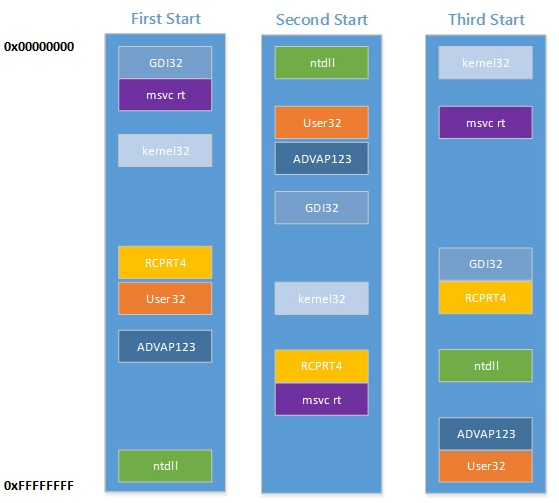
\includegraphics[width=\textwidth,height=\textheight,keepaspectratio]{sections/background/defenses/aslr.jpg}
\caption{ASLR resulting in different DLL memory locations after each boot}
\label{fig:aslr}
\end{figure}
The first of the built in windows defenses is called Address Space Layout Randomization \cite{miller2009method}. It's main purpose is to make memory allocations at a random address in the virtual address space. This is illustrated in Figure \ref{fig:aslr}, which shows three independent starts of the operating system represented by the three blue vertical bars. On the left, the address space is enumerated from the lowest to the highest possible address. The locations of the loaded DLL files is randomized on each start of Windows, and therefore the DLLs that can be seen inside each of the three columns have different positions. An attacker that tries to inject code into the application will no longer know which address has to be used. Searching inside the virtual address space is thus not feasible, as it is very large with four gigabyte on a 32 bit and eight terabyte on a 64 bit windows system of virtual addresses. Therefore the attacker might start duplicating his code several times to fill hundreds of addresses and by chance getting his code executed. As the main purpose of ASLR is to prevent buffer overflows, it is fulfilling its job by crashing the application due to an illegal memory access on not allocated memory. However, for all possible attacks, ASLR will not prevent all exploits \cite{shacham}. All methods involving \syscall{WriteProcessMemory} or DLL injection can use the Windows API function \syscall{GetProcAddress} to retrieve the address of an exported function. As the windows system is DLL dependent and procedures are exported from within DLLs, the attacker is granted an easy way to circumvent ASLR.